The performances of the A* based ESM is tested for two different test scenarios. In scenario 1 the system is tested against a Sampling-Based Model Predictive Control (SBMPC) scenerio (CITE DOCTDER JOURNAL). In scenario 2 the ESM is tested against two simple base test cases using PGNE test data.

\subsection{Comparison with SBMPC}
 Model predictive control (MPC) uses a predictive model to optimize a cost function while enforcing constraints on the sytem inputs and outputs and is widely applied in industrial process control \cite{qin1997overview}. Typically, industrial MPC is implemented for linear models, but the use of nonlinear models allows better performance over a wider operating range \cite{berber2012nonlinear}. SBMPC \cite{dunlap2011book}, \cite{reese2016graph} is an MPC method that uses a receding horizon along with the optimization algorithm, Sampling-Based Model Predictive Optimization (SBMPO), which samples the input of the predictive model to compute a  graph tree with nodes and branches. Figure \ref{fig:EMS_7_7days} shows the response of the EMS for 7 days.
 
 \begin{figure}[!ht]
    \centering
    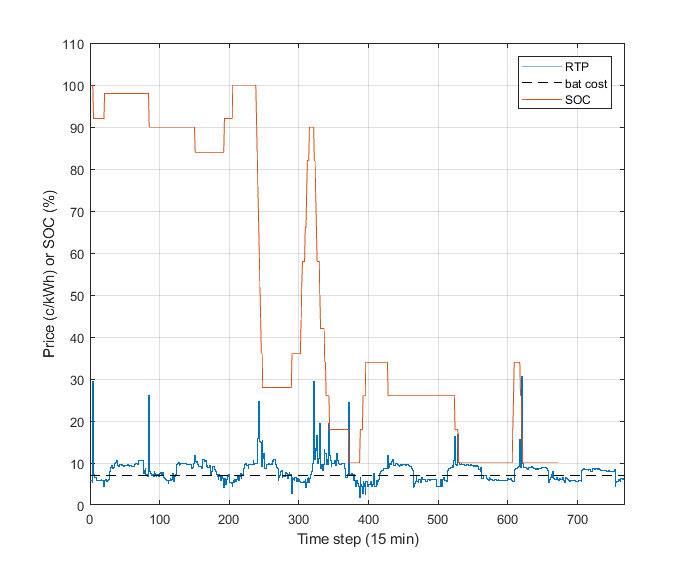
\includegraphics[width = \linewidth]{figs/Plot100_7.png}
    \caption{EMS response}
    \label{fig:EMS_7_7days}
\end{figure}

\subsection{PG\&E peak day pricing test result}

Figure \ref{fig:EMS_7_PGNE} shows the PGNE test results for the 7 days.

\begin{figure}[!ht]
    \centering
    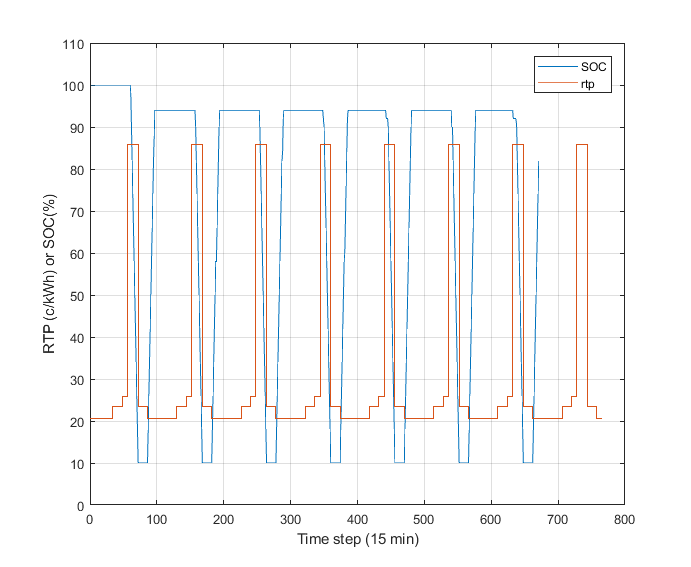
\includegraphics[width = \linewidth]{figs/PGNE_PEAK_100_7_24.png}
    \caption{EMS response}
    \label{fig:EMS_7_PGNE}
\end{figure}
